\documentclass[11pt]{article}
\usepackage[margin=0.85in]{geometry}
\usepackage{amsmath,amssymb,mathtools,enumitem,booktabs}
\usepackage[T1]{fontenc}
\usepackage{lmodern}
\usepackage{pgfplots}
\pgfplotsset{compat=1.18}
\usepackage[colorlinks=true,linkcolor=blue]{hyperref}
\newcommand{\ex}[1]{\subsection*{#1.}}
\newcommand{\ans}[1]{\boxed{#1}}
\newcommand{\vv}[1]{\left\langle #1\right\rangle}
\newcommand{\ii}{\mathbf i}\newcommand{\jj}{\mathbf j}\newcommand{\kk}{\mathbf k}
\newcommand{\cp}[6]{\begin{vmatrix}\ii&\jj&\kk\\#1&#2&#3\\#4&#5&#6\end{vmatrix}}
\pgfplotsset{every axis/.append style={width=.70\linewidth,height=6cm,xlabel={$x$},ylabel={$y$},zlabel={$z$},view={125}{25},grid=major}}
\newcommand{\surf}[4]{\begin{center}\begin{tikzpicture}\begin{axis}[#1]\addplot3[surf,shader=interp,samples=19,samples y=19,opacity=.78] ({#2},{#3},{#4});\end{axis}\end{tikzpicture}\end{center}}
\newcommand{\curve}[4]{\begin{center}\begin{tikzpicture}\begin{axis}[#1]\addplot3[blue,thick,samples=180,samples y=0,variable=t] ({#2},{#3},{#4});\end{axis}\end{tikzpicture}\end{center}}
\newcommand{\field}[2]{\begin{center}\begin{tikzpicture}\begin{axis}[view={0}{90},axis equal image,domain=-2:2,y domain=-2:2,samples=6,samples y=6,xmin=-2.6,xmax=2.6,ymin=-2.6,ymax=2.6]\addplot3[blue,quiver={u={#1},v={#2},w=0,scale arrows=.22},-stealth] {0};\end{axis}\end{tikzpicture}\end{center}}
\title{Chapter 16: Vector Calculus\\Worked solutions to the assigned exercises}
\author{}\date{}\begin{document}\maketitle
\noindent Source: Stewart, Clegg, and Watson, ninth edition. Exercises follow the supplied assignment screenshot. Arrow lengths in sketches are scaled uniformly for readability.
\tableofcontents
\clearpage\section*{16.1: Vector fields}\addcontentsline{toc}{section}{16.1: Vector fields}
\ex{1}
$\mathbf F=\vv{1,1/2}$ is constant: every arrow points right and upward, with slope $1/2$. Its magnitude is
\[\sqrt{1+1/4}=\sqrt5/2.\] For example, the vectors based at $(0,0)$, $(1,0)$, and $(0,1)$ all have identical components.
\field{1}{.5}
\ex{3}
$\mathbf F=\vv{1,y/2}$ always has rightward horizontal component 1. It points up for $y>0$, right on $y=0$, and down for $y<0$. The magnitude $\sqrt{1+y^2/4}$ grows with $|y|$, and the field is constant along each horizontal line. At heights $-2,0,2$, the vectors are $\vv{1,-1}$, $\vv{1,0}$, and $\vv{1,1}$.
\field{1}{y/2}
\ex{5}
$\mathbf F=\vv{-1/2,y-x}$ always points left. Its vertical component vanishes on $y=x$, is positive above that line, and negative below it. At $(0,1)$ the vector is $\vv{-1/2,1}$; at $(1,0)$ it is $\vv{-1/2,-1}$. Vectors along $y=x$ are horizontal with length $1/2$.
\field{-.5}{y-x}
\ex{7}
For $(x,y)\ne(0,0)$,
\[\mathbf F=\frac{\vv{y,x}}{\sqrt{x^2+y^2}},\qquad
|\mathbf F|=\sqrt{\frac{y^2+x^2}{x^2+y^2}}=1.\]
Thus every arrow has unit length. On positive $x$, arrows point up; on positive $y$, they point right. On the negative axes, these directions reverse. At $(1,1)$ the arrow points northeast, while at $(1,-1)$ it points northwest. The field is undefined at the origin; no vector should be placed there.
\field{y/sqrt(x*x+y*y)}{x/sqrt(x*x+y*y)}
\ex{9}
$\mathbf F(x,y,z)=\ii=\vv{1,0,0}$ is constant in three dimensions. Every arrow is parallel to the positive $x$ axis, with length 1, regardless of its base point.
\begin{center}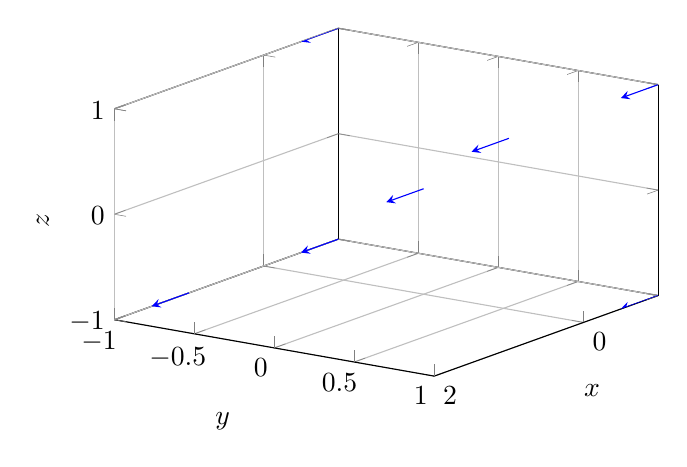
\begin{tikzpicture}\begin{axis}[xmin=-1,xmax=2,ymin=-1,ymax=1,zmin=-1,zmax=1]
\addplot3[blue,quiver={u=1,v=0,w=0,scale arrows=.5},-stealth] coordinates {(-1,-1,-1) (-1,1,-1) (-1,-1,1) (-1,1,1) (0,0,0) (1,-1,-1) (1,1,1)};
\end{axis}\end{tikzpicture}\end{center}
\ex{21}
$\mathbf F=\vv{x,y,3}$ has a constant upward component and horizontally points away from the $z$ axis. On the axis it is vertical; farther from the axis it tilts outward. Its magnitude $\sqrt{x^2+y^2+9}$ is independent of height. The matching picture is $\ans{\text{III}}$: all arrows point upward and the horizontal components spread outward.
\ex{25}
For $f=y\sin(xy)$, the chain rule gives $f_x=y\cos(xy)\,y=y^2\cos(xy)$. The product rule gives $f_y=\sin(xy)+y\cos(xy)\,x$. Therefore
\[\ans{\nabla f=\vv{y^2\cos(xy),\sin(xy)+xy\cos(xy)}}.\]
\clearpage\section*{16.2: Line integrals}\addcontentsline{toc}{section}{16.2: Line integrals}
A scalar arc-length integral uses $ds=|\mathbf r'(t)|dt$, while an oriented vector integral uses $d\mathbf r=\mathbf r'(t)dt$. In particular, $Pdx+Qdy+Rdz$ uses the signed coordinate derivatives, not their magnitudes.
\ex{1}
With $x=t^2$, $y=2t$, $0\le t\le3$, $\mathbf r'=\vv{2t,2}$, so $ds=2\sqrt{t^2+1}dt$. Thus
\[I=\int_0^3(2t)2\sqrt{t^2+1}dt.\]
Set $u=t^2+1$, $du=2t\,dt$; the limits become 1 and 10:
\[I=2\int_1^{10}\sqrt u\,du=\frac43[u^{3/2}]_1^{10}=\ans{\frac43(10\sqrt{10}-1)}.\]
\ex{3}
The right semicircle is $x=4\cos t$, $y=4\sin t$, $-\pi/2\le t\le\pi/2$. Its speed is $\sqrt{16\sin^2t+16\cos^2t}=4$, so
\[I=\int_{-\pi/2}^{\pi/2}(4\cos t)(4\sin t)^4(4)dt
=4096\int_{-\pi/2}^{\pi/2}\cos t\sin^4t\,dt.\]
With $u=\sin t$, $du=\cos t\,dt$, this is $4096[u^5/5]_{-1}^1=\ans{8192/5}$.
\ex{5}
Use $x=t$, $y=t^2$, $0\le t\le\pi$; then $dy=2t\,dt$:
\[I=\int_0^\pi(t^4+\sin t)2t\,dt=2\int_0^\pi t^5dt+2\int_0^\pi t\sin t\,dt.\]
For the second term, integration by parts gives $\int t\sin t\,dt=-t\cos t+\sin t$. Hence
\[I=[t^6/3]_0^\pi+2[-t\cos t+\sin t]_0^\pi=\ans{\pi^6/3+2\pi}.\]
\ex{7}
The first segment, from $(0,0)$ to $(2,1)$, is $(x,y)=(2t,t)$, $0\le t\le1$. Thus $dx=2dt$, $dy=dt$, and
\[I_1=\int_0^1[(2t+2t)2+(2t)^2]dt=[4t^2+4t^3/3]_0^1=16/3.\]
The second segment, from $(2,1)$ to $(3,0)$, is $(x,y)=(2+t,1-t)$, with $dx=dt$, $dy=-dt$:
\[I_2=\int_0^1[(2+t+2-2t)-(2+t)^2]dt
=\int_0^1(-5t-t^2)dt=-5/2-1/3=-17/6.\]
Adding gives $\ans{I=16/3-17/6=5/2}$.
\ex{9}
For $\mathbf r(t)=\vv{\cos t,\sin t,t}$, $0\le t\le\pi/2$, the derivative is $\vv{-\sin t,\cos t,1}$ and its magnitude is $\sqrt2$. Therefore
\[I=\sqrt2\int_0^{\pi/2}\cos t\sin^2t\,dt
=\sqrt2[\sin^3t/3]_0^{\pi/2}=\ans{\sqrt2/3}.\]
\ex{11}
Parametrize the segment by $\mathbf r(t)=\vv{t,2t,3t}$, $0\le t\le1$. Then $|\mathbf r'|=\sqrt{1+4+9}=\sqrt{14}$ and $xe^{yz}=te^{6t^2}$. Thus
\[I=\sqrt{14}\int_0^1te^{6t^2}dt=\frac{\sqrt{14}}{12}[e^{6t^2}]_0^1=\ans{\sqrt{14}(e^6-1)/12}.\]
Here the substitution $u=6t^2$ gives $du=12t\,dt$.
\ex{13}
With $x=t$, $y=t^2$, $z=t^3$, $0\le t\le1$, we have $dy=2t\,dt$ and $yz=t^5$:
\[I=\int_0^1(t)(t^2)e^{t^5}(2t)dt=2\int_0^1t^4e^{t^5}dt.\]
Let $u=t^5$, $du=5t^4dt$. Then $I=(2/5)[e^u]_0^1=\ans{2(e-1)/5}$.
\ex{15}
The coordinate derivatives are $dx=\cos t\,dt$, $dy=-\sin t\,dt$, and $dz=\sec^2t\,dt$. Hence
\begin{align*}
I&=\int_{-\pi/4}^{\pi/4}[\tan t\cos t+\sin t\cos t(-\sin t)+\cos^2t\sec^2t]dt\\
&=\int_{-\pi/4}^{\pi/4}(\sin t-\sin^2t\cos t+1)dt.
\end{align*}
The sine term is odd and integrates to zero. An antiderivative of $\sin^2t\cos t$ is $\sin^3t/3$, giving
\[I=\pi/2-[\sin^3t/3]_{-\pi/4}^{\pi/4}
=\pi/2-\frac23(\sqrt2/2)^3=\ans{\pi/2-\sqrt2/6}.\]
\ex{19}
\textbf{(a)} Along the upward vertical segment $x=-3$, the pictured arrows have positive vertical component everywhere. The horizontal component contributes nothing because $dx=0$. Thus $\mathbf F\cdot d\mathbf r=F_y\,dy>0$ and the integral is $\ans{\text{positive}}$.
\textbf{(b)} The field circulates clockwise, so along the counterclockwise circle its tangential component is negative everywhere. Thus the integral is $\ans{\text{negative}}$.
\ex{21}
For $\mathbf r=\vv{t^3,t^2}$, $0\le t\le1$, $\mathbf r'=\vv{3t^2,2t}$. Substituting into $\mathbf F=\vv{xy^2,-x^2}$ gives $\mathbf F(\mathbf r)=\vv{t^7,-t^6}$. Taking the dot product,
\[I=\int_0^1[(t^7)(3t^2)+(-t^6)(2t)]dt
=\int_0^1(3t^9-2t^7)dt=[3t^{10}/10-t^8/4]_0^1=\ans{1/20}.\]

\clearpage\section*{16.3: The fundamental theorem for line integrals}\addcontentsline{toc}{section}{16.3: The fundamental theorem for line integrals}
If $\mathbf F=\nabla f$, the chain rule yields $\mathbf F(\mathbf r(t))\cdot\mathbf r'(t)=d[f(\mathbf r(t))]/dt$, so the integral equals $f(B)-f(A)$. In the plane, $P_y=Q_x$ is a necessary test; on a simply connected domain with continuous first partials it is also sufficient.
\ex{3}
Here $P=xy+y^2$, $Q=x^2+2xy$, so $P_y=x+2y$, whereas $Q_x=2x+2y$. They disagree, for example at $(1,0)$. Thus $\ans{\mathbf F\text{ is not conservative}}$ and no global potential exists.
\ex{5}
$P=y^2e^{xy}$, $Q=(1+xy)e^{xy}$. Differentiation gives
\[P_y=(2y+xy^2)e^{xy}=Q_x.\]
The domain is all of $\mathbb R^2$, so the field is conservative. Integrating $P$ with respect to $x$ gives $f=ye^{xy}+g(y)$; this formula also remains valid at $y=0$. Then $f_y=(1+xy)e^{xy}+g'(y)=Q$, so $g'=0$. Hence $\ans{f=ye^{xy}+C}$.
\ex{7}
For $P=ye^x+\sin y$, $Q=e^x+x\cos y$, $P_y=e^x+\cos y=Q_x$ throughout the plane. Integrate $P$ in $x$:
\[f=ye^x+x\sin y+g(y),\qquad f_y=e^x+x\cos y+g'(y).\]
Matching $Q$ requires $g'=0$. Thus $\ans{f=ye^x+x\sin y+C}$ and the field is conservative.
\ex{9}
$P_y=2y\cos x-\sin y=Q_x$, so the field is conservative on $\mathbb R^2$. Integrating $P=y^2\cos x+\cos y$ in $x$ gives $f=y^2\sin x+x\cos y+g(y)$. Its $y$ derivative is $2y\sin x-x\sin y+g'(y)$, so $g'=0$. Therefore $\ans{f=y^2\sin x+x\cos y+C}$.
\ex{13}
\textbf{(a)} The lower semicircle from $(-2,0)$ to $(2,0)$ is $x=-2\cos t$, $y=-2\sin t$, $0\le t\le\pi$, with $dx=2\sin t\,dt$, $dy=-2\cos t\,dt$. Substitution gives
\begin{align*}
I&=\int_0^\pi[(12\cos^2t+4\sin^2t)2\sin t+(8\cos t\sin t)(-2\cos t)]dt\\
&=\int_0^\pi8\sin t(\cos^2t+\sin^2t)dt
=8[-\cos t]_0^\pi=\ans{16}.
\end{align*}
\textbf{(b)} $P_y=2y=Q_x$. Integrating $P$ gives $f=x^3+xy^2+g(y)$; $f_y=2xy+g'(y)$ implies $g'=0$, so $\ans{f=x^3+xy^2+C}$.
\textbf{(c)} $I=f(2,0)-f(-2,0)=8-(-8)=\ans{16}$.
\textbf{(d)} Replace the semicircle with the horizontal segment $y=0$, $-2\le x\le2$. Since $dy=0$, $I=\int_{-2}^23x^2dx=[x^3]_{-2}^2=\ans{16}$.
\ex{15}
\textbf{(a)} For $P=ye^{xy}$, $Q=xe^{xy}$, $P_y=(1+xy)e^{xy}=Q_x$. A potential is $f=e^{xy}+C$, as verified by $f_x=ye^{xy}$ and $f_y=xe^{xy}$.
\textbf{(b)} At $t=0$, $(x,y)=(\sin0,e^{-1}(1-\cos0))=(0,0)$. At $t=1$, $(x,y)=(\sin(\pi/2),e^0(1-\cos\pi))=(1,2)$. Thus $I=e^{(1)(2)}-e^0=\ans{e^2-1}$.
\textbf{(c)} On the straight segment $x=s$, $y=2s$, $0\le s\le1$, $dx=ds$, $dy=2ds$. Hence
\[I=\int_0^1[(2s)e^{2s^2}+se^{2s^2}(2)]ds
=\int_0^14se^{2s^2}ds=[e^{2s^2}]_0^1=\ans{e^2-1}.\]
\ex{17}
\textbf{(a)} Integrating $f_x=2x$ gives $f=x^2+g(y)$; matching $f_y=4y$ gives $g=2y^2+C$. Thus
\[\ans{f=x^2+2y^2+C}.\]
\textbf{(b)} The stated endpoints give $I=f(1,1)-f(4,-2)=(1+2)-(16+8)=\ans{-21}$.
\ex{19}
\textbf{(a)} Integrating $f_x=x^2y^3$ gives $f=x^3y^3/3+g(y)$. Then $f_y=x^3y^2+g'(y)$, so $g'=0$. Hence $\ans{f=x^3y^3/3+C}$.
\textbf{(b)} The curve starts at $(0,0)$ and ends at $(1-2,1+2)=(-1,3)$. Therefore $I=(-1)^3(3)^3/3-0=\ans{-9}$.
\ex{31}
The pictured field has a tangential component circulating around the origin: arrows on the right point upward, those above point left, those on the left point downward, and those below point right. Traversing a loop counterclockwise gives positive tangential contributions around the loop. Such nonzero circulation contradicts the zero integral required for every closed curve in a conservative field. Thus the plot indicates $\ans{\text{not conservative}}$.
\ex{33}
The field $\vv{\sin y,1+x\cos y}$ has $P_y=\cos y=Q_x$ and is smooth throughout the plane. To explicitly establish the potential, integrate $P$ in $x$: $f=x\sin y+g(y)$. Then $f_y=x\cos y+g'(y)$, requiring $g'=1$. Thus $\ans{f=x\sin y+y+C}$ and the field is conservative. Its gradients point perpendicular to the contours $x\sin y+y=\text{constant}$.
\field{sin(deg(y))}{1+x*cos(deg(y))}
\ex{35}
Since $\mathbf F=\nabla f$, $P=f_x$, $Q=f_y$, $R=f_z$. The assumed continuous first derivatives of $P,Q,R$ are continuous second derivatives of $f$. Equality of mixed partial derivatives gives
\[P_y=f_{xy}=f_{yx}=Q_x,\quad
P_z=f_{xz}=f_{zx}=R_x,\quad
Q_z=f_{yz}=f_{zy}=R_y.\]
These are precisely the three required identities.

\clearpage\section*{16.4: Green's theorem}\addcontentsline{toc}{section}{16.4: Green's theorem}
For positive orientation (counterclockwise outer boundary), Green's theorem states $\oint_C Pdx+Qdy=\iint_D(Q_x-P_y)dA$. Inner boundaries of holes must be clockwise. If the given outer boundary is clockwise, reverse the sign.
\ex{1}
\textbf{(a)} Traverse the rectangle counterclockwise. On its bottom, $y=0$, so the integral is zero. On the right, $x=5$, $dx=0$, and $\int_0^425y\,dy=200$. On top, $y=4$, $dy=0$, and $\int_5^016dx=-80$. On the left, $x=0$, $dx=0$, so the integral is zero. The total is $\ans{120}$.
\textbf{(b)} $Q_x-P_y=2xy-2y=2y(x-1)$. Thus
\[I=\int_0^4\int_0^52y(x-1)dx\,dy
=\int_0^42y[x^2/2-x]_0^5dy=15\int_0^4y\,dy=\ans{120}.\]
\ex{3}
\textbf{(a)} On $(0,0)\to(1,0)$ the integrand vanishes. On $(1,0)\to(1,2)$, $x=1$, $dx=0$, so $I_2=\int_0^2y^3dy=4$. On the return segment, set $x=t$, $y=2t$, with $t$ decreasing from 1 to 0. Then $dx=dt$, $dy=2dt$:
\[I_3=\int_1^0[2t^2+(t^2)(8t^3)(2)]dt
=[2t^3/3+8t^6/3]_1^0=-10/3.\]
Hence $I=0+4-10/3=\ans{2/3}$.
\textbf{(b)} $Q_x-P_y=2xy^3-x$, and $D$ has $0\le x\le1$, $0\le y\le2x$. Therefore
\[I=\int_0^1\int_0^{2x}(2xy^3-x)dy\,dx
=\int_0^1[xy^4/2-xy]_0^{2x}dx
=\int_0^1(8x^5-2x^2)dx=\ans{2/3}.\]
\ex{5}
For $P=ye^x$, $Q=2e^x+2x^2$, $Q_x-P_y=(2e^x+4x)-e^x=e^x+4x$. Thus on $0\le x\le3$, $0\le y\le4$,
\[I=\int_0^3\int_0^4(e^x+4x)dy\,dx
=4[e^x+2x^2]_0^3=\ans{4e^3+68}.\]
\ex{7}
Here $P=x^2y^2$, $Q=\arctan y$, so $Q_x-P_y=0-2x^2y$. The triangle is $0\le x\le1$, $0\le y\le3x$:
\[I=\int_0^1\int_0^{3x}-2x^2y\,dy\,dx
=\int_0^1[-x^2y^2]_0^{3x}dx=-9\int_0^1x^4dx=\ans{-9/5}.\]
\ex{9}
For $P=y+e^{\sqrt x}$ and $Q=2x+\cos(y^2)$, the needed derivatives are $P_y=1$, $Q_x=2$, so the integrand is 1. The boundaries $y=x^2$, $x=y^2$ meet at $(0,0)$ and $(1,1)$; on $0\le x\le1$, $x^2\le y\le\sqrt x$. Thus
\[I=\int_0^1\int_{x^2}^{\sqrt x}1dy\,dx
=[2x^{3/2}/3-x^3/3]_0^1=\ans{1/3}.\]
Although $\partial P/\partial x$ is singular at $x=0$, the $e^{\sqrt x}dx$ term has a continuous one-variable antiderivative and integrates to zero around the closed boundary. Apply Green's theorem to the remaining smooth terms (or take an interior limiting region) to justify this evaluation.
\ex{11}
$Q_x-P_y=-3x^2-3y^2=-3r^2$. For the radius-2 disk,
\[I=-3\int_0^{2\pi}\int_0^2r^3dr\,d\theta
=-6\pi[r^4/4]_0^2=\ans{-24\pi}.\]
\ex{13}
The arrows give positive orientation of the first-quadrant annular sector: its outer arc is counterclockwise and its inner arc clockwise. Since $P=3+e^x$ and $Q=\arctan y+3x^2$, $Q_x-P_y=6x$. Thus
\[I=\int_0^{\pi/2}\int_1^26r^2\cos\theta\,dr\,d\theta
=6[r^3/3]_1^2[\sin\theta]_0^{\pi/2}=\ans{14}.\]
\ex{17}
$P=y-\cos y$, $Q=x\sin y$ gives $Q_x-P_y=\sin y-(1+\sin y)=-1$. The circle has radius 2 and is clockwise. Reversing Green's theorem's positive orientation gives
\[I=-\iint_D(-1)dA=\operatorname{area}(D)=\ans{4\pi}.\]
\ex{21}
The path $(0,0)\to(1,0)\to(0,1)\to(0,0)$ is counterclockwise. With $P=x(x+y)$, $Q=xy^2$, $Q_x-P_y=y^2-x$. The triangle has $0\le x\le1$, $0\le y\le1-x$:
\begin{align*}
W&=\int_0^1\int_0^{1-x}(y^2-x)dy\,dx\\
&=\int_0^1[(1-x)^3/3-x(1-x)]dx
=1/12-(1/2-1/3)=\ans{-1/12}.
\end{align*}
\ex{27}
Place the quarter disk in the first quadrant. Its area is $A=\pi a^2/4$. For the positive boundary, the axis segments contribute zero to $\oint x^2dy$ and $\oint y^2dx$. On the circular arc use $x=a\cos t$, $y=a\sin t$, $0\le t\le\pi/2$:
\[\oint x^2dy=a^3\int_0^{\pi/2}\cos^3t\,dt
=a^3[\sin t-\sin^3t/3]_0^{\pi/2}=2a^3/3,\]
\[\oint y^2dx=-a^3\int_0^{\pi/2}\sin^3t\,dt=-2a^3/3.\]
The centroid formulas therefore give
\[\bar x=\frac{2a^3/3}{2(\pi a^2/4)}=\frac{4a}{3\pi},\qquad
\bar y=-\frac{-2a^3/3}{2(\pi a^2/4)}=\frac{4a}{3\pi}.\]
Thus $\ans{(\bar x,\bar y)=(4a/(3\pi),4a/(3\pi))}$.
\ex{29}
For constant density $\rho$, $I_x=\rho\iint_Dy^2dA$ and $I_y=\rho\iint_Dx^2dA$. Choose $P=-y^3/3$, $Q=0$ for the first integral. Then $Q_x-P_y=y^2$, and Green's theorem gives
\[\ans{I_x=-\frac\rho3\oint_Cy^3dx}.\]
For the second, choose $P=0$, $Q=x^3/3$; then $Q_x-P_y=x^2$, giving
\[\ans{I_y=\frac\rho3\oint_Cx^3dy}.\]
The boundary is positively oriented in both formulas.

\clearpage\section*{16.5: Curl and divergence}\addcontentsline{toc}{section}{16.5: Curl and divergence}
For $\mathbf F=\vv{P,Q,R}$, expansion of the differential determinant gives
\[\nabla\times\mathbf F=\begin{vmatrix}\ii&\jj&\kk\\\partial_x&\partial_y&\partial_z\\P&Q&R\end{vmatrix}
=\ii(R_y-Q_z)-\jj(R_x-P_z)+\kk(Q_x-P_y).\]
Divergence is the scalar $\nabla\cdot\mathbf F=P_x+Q_y+R_z$.
\ex{1}
\textbf{(a)} For $\mathbf F=\vv{xy^2z^2,x^2yz^2,x^2y^2z}$,
\begin{align*}
\nabla\times\mathbf F
&=\begin{vmatrix}\ii&\jj&\kk\\\partial_x&\partial_y&\partial_z\\xy^2z^2&x^2yz^2&x^2y^2z\end{vmatrix}\\
&=\ii(2x^2yz-2x^2yz)-\jj(2xy^2z-2xy^2z)+\kk(2xyz^2-2xyz^2)=\ans{\mathbf0}.
\end{align*}
\textbf{(b)} $P_x=y^2z^2$, $Q_y=x^2z^2$, $R_z=x^2y^2$, so $\ans{\operatorname{div}\mathbf F=y^2z^2+x^2z^2+x^2y^2}$.
\ex{3}
\textbf{(a)} Here $P=xye^x$, $Q=yze^x$, $R=0$. Expanding,
\[\operatorname{curl}\mathbf F=\ii(0-ye^x)-\jj(0-0)+\kk(yze^x-xe^x)
=\ans{\vv{-ye^x,0,(yz-x)e^x}}.\]
\textbf{(b)} The product rule gives $P_x=y(1+x)e^x$, $Q_y=ze^x$, $R_z=0$. Thus $\ans{\operatorname{div}\mathbf F=(y+xy+z)e^x}$.
\ex{5}
Work in the differentiable domain $x,y,z>0$. \textbf{(a)} The relevant cross derivatives are
\[R_y=-\frac{\sqrt z}{(1+y)^2},\ Q_z=0,\ P_z=-\frac{\sqrt x}{(1+z)^2},\ R_x=0,\ Q_x=-\frac{\sqrt y}{(1+x)^2},\ P_y=0.\]
Substituting in the determinant expansion gives
\[\ans{\operatorname{curl}\mathbf F=\vv{-\sqrt z/(1+y)^2,-\sqrt x/(1+z)^2,-\sqrt y/(1+x)^2}}.\]
\textbf{(b)} Differentiating each numerator in its own coordinate gives
\[\ans{\operatorname{div}\mathbf F=\frac1{2\sqrt x(1+z)}+\frac1{2\sqrt y(1+x)}+\frac1{2\sqrt z(1+y)}}.\]
\ex{7}
\textbf{(a)} For $P=e^x\sin y$, $Q=e^y\sin z$, $R=e^z\sin x$, the curl expansion is
\[\ii(0-e^y\cos z)-\jj(e^z\cos x-0)+\kk(0-e^x\cos y),\]
so $\ans{\operatorname{curl}\mathbf F=\vv{-e^y\cos z,-e^z\cos x,-e^x\cos y}}$.
\textbf{(b)} $P_x=e^x\sin y$, $Q_y=e^y\sin z$, $R_z=e^z\sin x$, giving $\ans{\operatorname{div}\mathbf F=e^x\sin y+e^y\sin z+e^z\sin x}$.
\ex{12}
\textbf{(a)} The horizontal component is constant along horizontal lines, and the vertical component is constant along vertical lines. Thus the plot indicates $P_x=0$, $Q_y=0$, so $\ans{\operatorname{div}\mathbf F=0}$: a small box has balanced inflow and outflow.
\textbf{(b)} The arrows circulate counterclockwise. Their leftward component grows as $y$ increases ($P_y<0$), while the upward component grows as $x$ increases ($Q_x>0$). Therefore $Q_x-P_y>0$ and the curl is nonzero, pointing $\ans{\text{in the positive }z\text{ direction}}$.
\ex{13}
\textbf{(a)} For $f=\sin(xyz)$,
\[\nabla f=\vv{yz\cos(xyz),xz\cos(xyz),xy\cos(xyz)}.\]
To verify its curl vanishes, explicitly calculate the paired derivatives:
\[f_{zy}=x\cos(xyz)-x^2yz\sin(xyz)=f_{yz},\]
\[f_{zx}=y\cos(xyz)-xy^2z\sin(xyz)=f_{xz},\]
\[f_{yx}=z\cos(xyz)-xyz^2\sin(xyz)=f_{xy}.\]
Thus the determinant expansion $\ii(f_{zy}-f_{yz})-\jj(f_{zx}-f_{xz})+\kk(f_{yx}-f_{xy})$ is $\ans{\mathbf0}$.
\textbf{(b)} For $\mathbf F=\vv{xyz^2,x^2yz^3,y^2}$,
\[\operatorname{curl}\mathbf F=\vv{2y-3x^2yz^2,2xyz,2xyz^3-xz^2}.\]
Now differentiate these three components in $x,y,z$, respectively:
\[\operatorname{div}(\operatorname{curl}\mathbf F)
=(-6xyz^2)+(2xz)+(6xyz^2-2xz)=\ans{0}.\]
\ex{15}
Integrating $f_x=2xy^3z^2$ gives $f=x^2y^3z^2+g(y,z)$. Then $f_y=3x^2y^2z^2+g_y$ forces $g_y=0$, so $g=h(z)$. Finally $f_z=2x^2y^3z+h'$ forces $h'=0$. Hence $\ans{f=x^2y^3z^2+C}$; checking all three derivatives establishes that the field is conservative on $\mathbb R^3$.
\ex{17}
The real domain is $y>0$, $z>0$. Integrating $f_x=\ln y$ gives $f=x\ln y+g(y,z)$. Matching $f_y=x/y+\ln z$ gives $g_y=\ln z$, so $g=y\ln z+h(z)$. Then $f_z=y/z+h'(z)$ must equal $y/z$, so $h'=0$. Thus $\ans{f=x\ln y+y\ln z+C}$ and the field is conservative on its domain.
\ex{19}
For $P=yz^2e^{xz}$, $Q=ze^{xz}$, $R=xyze^{xz}$, the first curl component is
\[R_y-Q_z=xze^{xz}-(1+xz)e^{xz}=-e^{xz}.\]
It never vanishes. A conservative field would have zero curl; therefore $\ans{\mathbf F\text{ is not conservative}}$ and no potential exists.

\clearpage\section*{16.6: Parametric surfaces and their areas}\addcontentsline{toc}{section}{16.6: Parametric surfaces and their areas}
\ex{1}
For $P=(4,-5,1)$, solve $u+v=4$, $u-2v=-5$. Subtraction gives $3v=9$, so $v=3$, $u=1$. The third coordinate is $3+u-v=3+1-3=1$, so $\ans{P\text{ lies on the surface}}$.
For $Q=(0,4,6)$, the first two coordinates require $u+v=0$, $u-2v=4$. Thus $v=-4/3$, $u=4/3$, but $3+u-v=3+8/3=17/3\ne6$. Hence $\ans{Q\text{ does not lie on the surface}}$.
\ex{3}
From $x=u+v$, $y=3-v$, we obtain $v=3-y$, $u=x+y-3$. Substituting in $z=1+4u+5v$,
\[z=1+4(x+y-3)+5(3-y)=4x-y+4.\]
Thus the surface is the entire plane $\ans{z=4x-y+4}$. Every $(x,y)$ has corresponding real parameters, so the parametrization covers the whole plane.
\ex{5}
$x=s\cos t$, $y=s\sin t$, $z=s$ imply $x^2+y^2=s^2=z^2$. With unrestricted real $s$ the surface is the double circular cone $\ans{x^2+y^2=z^2}$. Positive $s$ covers the upper half, negative $s$ the lower half, and $s=0$ the vertex.
\ex{19}
Use the two given independent vectors as spanning directions:
\[\ans{\mathbf r(u,v)=u\vv{1,-1,0}+v\vv{0,1,0}=\vv{u,-u+v,0}},\quad u,v\in\mathbb R.\]
This is the $xy$ plane through the origin. Taking $u=x$ and $v=x+y$ reaches every point $(x,y,0)$.
\ex{21}
Rearrange the equation as $x^2=1+y^2+z^2/4$. The part in front of the $yz$ plane has $x>0$. Set $y=u$, $z=v$ and choose the positive square root:
\[\ans{\mathbf r(u,v)=\vv{\sqrt{1+u^2+v^2/4},u,v}},\quad u,v\in\mathbb R.\]
This selects the positive-$x$ sheet of the two-sheeted hyperboloid.
\ex{23}
Use spherical coordinates on the radius-2 sphere. The upward cone is $\phi=\pi/4$, so the portion above it is
\[\ans{\mathbf r(\theta,\phi)=\vv{2\sin\phi\cos\theta,2\sin\phi\sin\theta,2\cos\phi}},\quad0\le\theta<2\pi,\ 0\le\phi\le\pi/4.\]
The restriction includes its circular boundary and north pole.
\ex{25}
On the radius-6 sphere, $z=6\cos\phi$. The inequalities $0\le z\le3\sqrt3$ give $0\le\cos\phi\le\sqrt3/2$, so $\pi/6\le\phi\le\pi/2$. Hence
\[\ans{\mathbf r(\theta,\phi)=\vv{6\sin\phi\cos\theta,6\sin\phi\sin\theta,6\cos\phi}},\quad0\le\theta<2\pi,\ \pi/6\le\phi\le\pi/2.\]
\ex{33}
At $(2,3,0)$, $u+v=2$, $u-v=0$ give $u=v=1$, consistent with $3u^2=3$. The tangent vectors are $\mathbf r_u=\vv{1,6u,1}$ and $\mathbf r_v=\vv{1,0,-1}$. At $(1,1)$,
\begin{align*}
\mathbf n&=\cp{1}{6}{1}{1}{0}{-1}
=\ii(6(-1)-1(0))-\jj(1(-1)-1(1))+\kk(1(0)-6(1))\\
&=\vv{-6,2,-6}.
\end{align*}
The tangent plane is $-6(x-2)+2(y-3)-6z=0$, or $\ans{3x-y+3z=3}$.
\ex{39}
Write the plane as $z=6-3x-2y$, with $\mathbf r(x,y)=\vv{x,y,6-3x-2y}$. Its tangent vectors are $\vv{1,0,-3}$, $\vv{0,1,-2}$, and
\[\mathbf r_x\times\mathbf r_y=\cp{1}{0}{-3}{0}{1}{-2}
=\ii(0(-2)-(-3)(1))-\jj(1(-2)-(-3)(0))+\kk(1(1)-0(0))=\vv{3,2,1}.\]
The magnitude is $\sqrt{9+4+1}=\sqrt{14}$. The first-octant projection is the triangle $x\ge0$, $y\ge0$, $3x+2y\le6$, with intercepts 2 and 3. Therefore
\[A=\int_0^2\int_0^{3-3x/2}\sqrt{14}\,dy\,dx
=\sqrt{14}[3x-3x^2/4]_0^2=\ans{3\sqrt{14}}.\]
\ex{45}
Parametrize by $\mathbf r(x,y)=\vv{x,y,xy}$ on the unit disk. Then $\mathbf r_x=\vv{1,0,y}$, $\mathbf r_y=\vv{0,1,x}$, and
\[\mathbf r_x\times\mathbf r_y=\cp{1}{0}{y}{0}{1}{x}
=\ii(0x-y)-\jj(x-0)+\kk(1-0)=\vv{-y,-x,1}.\]
Thus $|\mathbf r_x\times\mathbf r_y|=\sqrt{1+x^2+y^2}$. In polar coordinates,
\[A=\int_0^{2\pi}\int_0^1\sqrt{1+r^2}\,r\,dr\,d\theta
=2\pi[(1+r^2)^{3/2}/3]_0^1=\ans{\frac{2\pi}{3}(2\sqrt2-1)}.\]
The radial antiderivative follows from $u=1+r^2$, $du=2rdr$.
\ex{61}
Complete the square: $x^2+y^2+(z-2)^2=4$, a sphere of radius 2 centered at $(0,0,2)$. Inside the paraboloid means $x^2+y^2\le z$. On the sphere, $r^2=4z-z^2$, so $4z-z^2\le z$, or $z(z-3)\ge0$. Since $0\le z\le4$, the surface portion is $3\le z\le4$, together with the isolated origin (which has zero area).
Parametrize the cap by
\[\mathbf r(\phi,\theta)=\vv{2\sin\phi\cos\theta,2\sin\phi\sin\theta,2+2\cos\phi},\quad0\le\phi\le\pi/3,\quad0\le\theta\le2\pi.\]
The tangent vectors are $\vv{2\cos\phi\cos\theta,2\cos\phi\sin\theta,-2\sin\phi}$ and $\vv{-2\sin\phi\sin\theta,2\sin\phi\cos\theta,0}$. Expanding their cross product gives
\begin{align*}
\mathbf r_\phi\times\mathbf r_\theta
&=\cp{2\cos\phi\cos\theta}{2\cos\phi\sin\theta}{-2\sin\phi}{-2\sin\phi\sin\theta}{2\sin\phi\cos\theta}{0}\\
&=\ii(4\sin^2\phi\cos\theta)-\jj(-4\sin^2\phi\sin\theta)
+\kk(4\sin\phi\cos\phi(\cos^2\theta+\sin^2\theta))\\
&=4\sin\phi\vv{\sin\phi\cos\theta,\sin\phi\sin\theta,\cos\phi}.
\end{align*}
The vector in brackets has unit length, so the area factor is $4\sin\phi$. Hence
\[A=\int_0^{2\pi}\int_0^{\pi/3}4\sin\phi\,d\phi\,d\theta
=8\pi(1-\cos(\pi/3))=\ans{4\pi}.\]
\surf{domain=0:360,y domain=0:60}{2*sin(y)*cos(x)}{2*sin(y)*sin(x)}{2+2*cos(y)}

\clearpage\section*{16.7: Surface integrals}\addcontentsline{toc}{section}{16.7: Surface integrals}
For a parametrization $\mathbf r(u,v)$, scalar integrals use $dS=|\mathbf r_u\times\mathbf r_v|du\,dv$. Flux integrals use the oriented vector $d\mathbf S=\pm(\mathbf r_u\times\mathbf r_v)du\,dv$. Choose the sign to match the prescribed normal.
\ex{5}
$\mathbf r=\vv{u+v,u-v,1+2u+v}$, $0\le u\le2$, $0\le v\le1$. Its tangent vectors are $\vv{1,1,2}$ and $\vv{1,-1,1}$. Expanding,
\[\mathbf r_u\times\mathbf r_v=\cp{1}{1}{2}{1}{-1}{1}
=\ii(1+2)-\jj(1-2)+\kk(-1-1)=\vv{3,1,-2}.\]
The magnitude is $\sqrt{9+1+4}=\sqrt{14}$ and $x+y+z=1+4u+v$. Hence
\[I=\sqrt{14}\int_0^2\int_0^1(1+4u+v)dv\,du
=\sqrt{14}\int_0^2(3/2+4u)du=\ans{11\sqrt{14}}.\]
\ex{7}
For $\mathbf r=\vv{u\cos v,u\sin v,v}$, the tangent vectors are $\vv{\cos v,\sin v,0}$ and $\vv{-u\sin v,u\cos v,1}$. Thus
\[\mathbf r_u\times\mathbf r_v=\cp{\cos v}{\sin v}{0}{-u\sin v}{u\cos v}{1}
=\ii(\sin v)-\jj(\cos v)+\kk(u\cos^2v+u\sin^2v)=\vv{\sin v,-\cos v,u}.\]
Its magnitude is $\sqrt{1+u^2}$. Since $y=u\sin v$,
\[I=\int_0^\pi\int_0^1u\sin v\sqrt{1+u^2}du\,dv
=2[(1+u^2)^{3/2}/3]_0^1=\ans{\frac23(2\sqrt2-1)}.\]
\ex{9}
$\mathbf r=\vv{x,y,1+2x+3y}$ has tangent vectors $\vv{1,0,2}$ and $\vv{0,1,3}$. Their cross product is
\[\cp{1}{0}{2}{0}{1}{3}=\ii(0-2)-\jj(3-0)+\kk(1-0)=\vv{-2,-3,1},\]
with magnitude $\sqrt{14}$. Therefore
\begin{align*}
I&=\sqrt{14}\int_0^3\int_0^2(x^2y+2x^3y+3x^2y^2)dy\,dx\\
&=\sqrt{14}\int_0^3(2x^2+4x^3+8x^2)dx
=\sqrt{14}[10x^3/3+x^4]_0^3=\ans{171\sqrt{14}}.
\end{align*}
\ex{11}
The triangle lies on $x-y/2+z/4=1$, so parametrize by $\vv{x,y,4-4x+2y}$. Its normal factor is
\[\cp{1}{0}{-4}{0}{1}{2}=\ii(0+4)-\jj(2-0)+\kk(1-0)=\vv{4,-2,1},\]
with magnitude $\sqrt{21}$. The projection has $0\le x\le1$, $2x-2\le y\le0$. Hence
\[I=\sqrt{21}\int_0^1\int_{2x-2}^0x\,dy\,dx
=\sqrt{21}\int_0^1(2x-2x^2)dx=\ans{\sqrt{21}/3}.\]
\ex{13}
Parametrize $x=y^2+z^2$ by $\mathbf r(y,z)=\vv{y^2+z^2,y,z}$ on $y^2+z^2\le1$. Then
\[\mathbf r_y\times\mathbf r_z=\cp{2y}{1}{0}{2z}{0}{1}
=\ii(1)-\jj(2y)+\kk(-2z)=\vv{1,-2y,-2z}.\]
The magnitude is $\sqrt{1+4y^2+4z^2}$. Set $y=r\cos\theta$, $z=r\sin\theta$:
\[I=\int_0^{2\pi}\int_0^1r^3\sin^2\theta\sqrt{1+4r^2}dr\,d\theta
=\pi\int_0^1r^3\sqrt{1+4r^2}dr.\]
For $w=1+4r^2$, $r^3dr=(w-1)dw/32$, so
\[I=\frac\pi{32}[2w^{5/2}/5-2w^{3/2}/3]_1^5=\ans{\pi(25\sqrt5+1)/120}.\]
\ex{15}
Use $\mathbf r(x,z)=\vv{x,x^2+4z,z}$ on the unit square. The area vector is
\[\cp{1}{2x}{0}{0}{4}{1}=\ii(2x)-\jj(1)+\kk(4)=\vv{2x,-1,4},\]
with magnitude $\sqrt{17+4x^2}$. Thus
\[I=\int_0^1\int_0^1x\sqrt{17+4x^2}dz\,dx
=[(17+4x^2)^{3/2}/12]_0^1=\ans{(21\sqrt{21}-17\sqrt{17})/12}.\]
The antiderivative uses $w=17+4x^2$, $dw=8x\,dx$.
\ex{17}
On the upper radius-2 hemisphere, $x=2\sin\phi\cos\theta$, $y=2\sin\phi\sin\theta$, $z=2\cos\phi$, $0\le\phi\le\pi/2$. The spherical cross product derived in Exercise 16.6.61 has magnitude $4\sin\phi$ (translation of a sphere does not change its tangent vectors). Since $(x^2+y^2)z=8\sin^2\phi\cos\phi$,
\[I=\int_0^{2\pi}\int_0^{\pi/2}32\sin^3\phi\cos\phi\,d\phi\,d\theta
=64\pi[\sin^4\phi/4]_0^{\pi/2}=\ans{16\pi}.\]
\ex{19}
Reflection $(x,y,z)\mapsto(x,y,-z)$ preserves every part of the closed cylinder boundary, including the two planar caps $x=0$ and $x+y=5$. It also preserves area. The integrand $xz$ changes sign. Pairing each point with its reflection cancels the contributions, so $\ans{I=0}$.
\ex{21}
The upward area vector for the parallelogram of Exercise 16.7.5 is the negative of its computed cross product: $\vv{-3,-1,2}$. For $\mathbf F=\vv{ze^{xy},-3ze^{xy},xy}$,
\[\mathbf F\cdot\vv{-3,-1,2}=-3ze^{xy}+3ze^{xy}+2xy=2xy=2(u^2-v^2).\]
Consequently
\[\Phi=\int_0^2\int_0^12(u^2-v^2)dv\,du
=2\int_0^2(u^2-1/3)du=2(8/3-2/3)=\ans{4}.\]
\ex{23}
For $z=4-x^2-y^2$, $\mathbf r_x=\vv{1,0,-2x}$ and $\mathbf r_y=\vv{0,1,-2y}$. The upward area vector is
\[\cp{1}{0}{-2x}{0}{1}{-2y}=\ii(2x)-\jj(-2y)+\kk(1)=\vv{2x,2y,1}.\]
Thus for $\mathbf F=\vv{xy,yz,zx}$,
\[\mathbf F\cdot\mathbf n\,dS=[2x^2y+2y^2(4-x^2-y^2)+x(4-x^2-y^2)]dx\,dy.\]
Integrating over $0\le x\le1$, $1\le y\le2$ gives
\[\Phi=\int_0^1\left(-x^3-\frac53x^2+\frac53x+\frac{94}{15}\right)dx
=\left[-x^4/4-5x^3/9+5x^2/6+94x/15\right]_0^1
=\ans{1133/180}.\]
\ex{25}
The outward unit normal of the unit sphere is $\mathbf n=\vv{x,y,z}$. Hence $\mathbf F\cdot\mathbf n=x^2+y^2+z^3$. The integral of $z^3$ vanishes by reflection across $z=0$. Rotational symmetry gives equal integrals of $x^2,y^2,z^2$; their sum equals the integral of 1 over the sphere, namely $4\pi$. Thus each is $4\pi/3$, and $\ans{\Phi=8\pi/3}$.
\ex{27}
The closed surface bounds $x^2+z^2\le y\le1$. On its paraboloid use $\mathbf r(x,z)=\vv{x,x^2+z^2,z}$. Its cross product is
\[\cp{1}{2x}{0}{0}{2z}{1}=\ii(2x)-\jj(1)+\kk(2z)=\vv{2x,-1,2z},\]
which points outward because the enclosed region is above the paraboloid. For $\mathbf F=\vv{0,y,-z}$, its dot product is $-y-2z^2=-x^2-3z^2$. On the unit disk in the $xz$ plane,
\[\Phi_1=-\int_0^{2\pi}\int_0^1r^3(\cos^2\theta+3\sin^2\theta)dr\,d\theta
=-\frac14(\pi+3\pi)=-\pi.\]
The upper disk $y=1$ has outward normal $\jj$, so $\mathbf F\cdot\jj=1$ and $\Phi_2=\pi$. Hence $\ans{\Phi=0}$.
\ex{29}
On the two $x$ faces the outward normals are $\pm\ii$, so $\mathbf F\cdot\mathbf n=1$ on both; each has area 4, contributing 8 together. On the two $y$ faces the value is 2, contributing $2(4)(2)=16$. On the two $z$ faces it is 3, contributing $2(4)(3)=24$. Therefore $\ans{\Phi=8+16+24=48}$.
\ex{31}
The boundary has two half-disk ends, a curved half-cylinder, and a bottom rectangle. At $x=0$, $\mathbf F\cdot(-\ii)=-x^2=0$; at $x=2$, it is 4, contributing $4(\pi/2)=2\pi$. At $z=0$, the downward flux is $-z^2=0$.
On the curved part use $\mathbf r(\theta,x)=\vv{x,\cos\theta,\sin\theta}$, $0\le\theta\le\pi$, $0\le x\le2$. Its tangent vectors are $\vv{0,-\sin\theta,\cos\theta}$ and $\vv{1,0,0}$, so
\[\cp{0}{-\sin\theta}{\cos\theta}{1}{0}{0}
=\ii(0)-\jj(-\cos\theta)+\kk(\sin\theta)=\vv{0,\cos\theta,\sin\theta},\]
which points outward. The dot product is $\cos^3\theta+\sin^3\theta$. The cosine term cancels over $[0,\pi]$, while
\[\int_0^\pi\sin^3\theta d\theta=[-\cos\theta+\cos^3\theta/3]_0^\pi=4/3.\]
The curved flux is $2(4/3)=8/3$, so $\ans{\Phi=2\pi+8/3}$.

\clearpage\section*{16.8: Stokes' theorem}\addcontentsline{toc}{section}{16.8: Stokes' theorem}
Stokes' theorem equates $\iint_S(\nabla\times\mathbf F)\cdot d\mathbf S$ with the circulation around the positively oriented boundary. It therefore permits replacing a surface with any convenient surface having the same oriented boundary.
\ex{1}
The disk, hemisphere, and paraboloid portion share the same boundary circle. Give each the orientation inducing the same direction around that circle. Applying Stokes' theorem to each gives the identical boundary integral $\oint_C\mathbf F\cdot d\mathbf r$; hence all three curl fluxes agree. Their different shapes and areas do not affect this equality.
\ex{3}
Replace the hemisphere by the radius-4 disk $y=0$ with normal $+\jj$. For $P=ze^y$, $Q=x\cos y$, $R=xz\sin y$, expand
\[\operatorname{curl}\mathbf F=\ii(xz\cos y-0)-\jj(z\sin y-e^y)+\kk(\cos y-ze^y).\]
At $y=0$, the $y$ component is $e^0-z\sin0=1$. Thus
\[\iint_S\operatorname{curl}\mathbf F\cdot d\mathbf S
=\iint_{x^2+z^2\le16}1\,dx\,dz=\ans{16\pi}.\]
\ex{5}
The five outward cube faces have the same oriented boundary as the bottom square with upward normal. Indeed the downward bottom would close the cube, making its boundary cancel the boundary of the five faces. For $\mathbf F=\vv{xyz,xy,x^2yz}$,
\[\operatorname{curl}\mathbf F
=\ii(x^2z-0)-\jj(2xyz-xy)+\kk(y-xz).\]
On the replacement bottom $z=-1$, the upward component is $y+x$. Therefore
\[I=\int_{-1}^1\int_{-1}^1(x+y)dx\,dy=\ans{0},\]
by odd symmetry of each summand over the square.
\ex{7}
For $\mathbf F=\vv{x+y^2,y+z^2,z+x^2}$,
\[\operatorname{curl}\mathbf F=\ii(0-2z)-\jj(2x-0)+\kk(0-2y)=\vv{-2z,-2x,-2y}.\]
Use the triangular plane $z=1-x-y$ with upward orientation. Its area vector is
\[\cp{1}{0}{-1}{0}{1}{-1}=\ii(1)-\jj(-1)+\kk(1)=\vv{1,1,1}.\]
The dot product is $-2(z+x+y)=-2$. The projection is $0\le x\le1$, $0\le y\le1-x$, so
\[I=\int_0^1\int_0^{1-x}(-2)dy\,dx=-2[x-x^2/2]_0^1=\ans{-1}.\]
\ex{9}
For $\mathbf F=\vv{xy,yz,zx}$, the curl determinant expands to $\ii(0-y)-\jj(z-0)+\kk(0-x)=\vv{-y,-z,-x}$. The upward area vector of $z=1-x^2-y^2$ is
\[\cp{1}{0}{-2x}{0}{1}{-2y}=\ii(2x)-\jj(-2y)+\kk(1)=\vv{2x,2y,1}.\]
Their dot product is $-2xy-2y(1-x^2-y^2)-x$. On the quarter unit disk, use $x=r\cos\theta$, $y=r\sin\theta$:
\begin{align*}
I&=-2\left(\int_0^1r^3dr\right)\left(\int_0^{\pi/2}\cos\theta\sin\theta d\theta\right)\\
&\quad-2\left(\int_0^1(r^2-r^4)dr\right)\left(\int_0^{\pi/2}\sin\theta d\theta\right)
-\left(\int_0^1r^2dr\right)\left(\int_0^{\pi/2}\cos\theta d\theta\right)\\
&=-2(1/4)(1/2)-2(1/3-1/5)(1)-(1/3)(1)=\ans{-17/20}.
\end{align*}
\ex{11}
\textbf{(a)} Use the radius-2 disk in $z=0$ with upward normal. The only required component of the curl of $\vv{-yx^2,xy^2,e^{xy}}$ is
\[(\operatorname{curl}\mathbf F)_z=Q_x-P_y=y^2-(-x^2)=x^2+y^2.\]
Thus Stokes' theorem gives
\[I=\int_0^{2\pi}\int_0^2r^3dr\,d\theta=2\pi[r^4/4]_0^2=\ans{8\pi}.\]
\ex{13}
The curve lies in $z=y$. Its projection $(\cos t,\sin t)$ traverses the unit circle counterclockwise, so choose the upward plane disk. The curl is
\[\operatorname{curl}\mathbf F=\ii(0-0)-\jj(0-0)+\kk(3x^2-x^2)=\vv{0,0,2x^2}.\]
The plane parametrization $\vv{x,y,y}$ has area vector
\[\cp{1}{0}{0}{0}{1}{1}=\ii(0)-\jj(1)+\kk(1)=\vv{0,-1,1}.\]
Therefore
\[I=\iint_{x^2+y^2\le1}2x^2dA
=2\int_0^1r^3dr\int_0^{2\pi}\cos^2\theta d\theta=\ans{\pi/2}.\]
\ex{15}
\textbf{(a)} The plane is $z=1-x-y$, and its upward area vector is $\vv{1,1,1}$, as expanded in Exercise 16.8.7. For $\mathbf F=\vv{x^2z,xy^2,z^2}$,
\[\operatorname{curl}\mathbf F=\ii(0-0)-\jj(0-x^2)+\kk(y^2-0)=\vv{0,x^2,y^2}.\]
The dot product is $x^2+y^2$, and the projection is the radius-3 disk. Thus
\[I=\int_0^{2\pi}\int_0^3r^3dr\,d\theta=2\pi[r^4/4]_0^3=\ans{81\pi/2}.\]
\textbf{(b)} The following plot shows the plane disk bounded by the cylinder, together with a portion of the cylinder. The disk has the upward orientation used above.
\begin{center}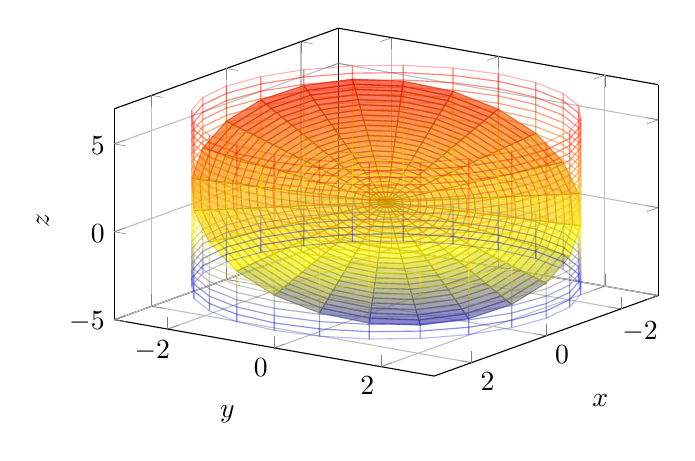
\begin{tikzpicture}\begin{axis}
\addplot3[surf,opacity=.65,domain=0:360,y domain=0:3,samples=25] ({y*cos(x)},{y*sin(x)},{1-y*cos(x)-y*sin(x)});
\addplot3[mesh,opacity=.3,domain=0:360,y domain=-4:6,samples=25] ({3*cos(x)},{3*sin(x)},{y});
\end{axis}\end{tikzpicture}\end{center}
\textbf{(c)} Parametrize the cylinder's circular projection and substitute into the plane:
\[\ans{\mathbf r(t)=\vv{3\cos t,3\sin t,1-3\cos t-3\sin t}},\quad0\le t\le2\pi.\]
Increasing $t$ gives the required counterclockwise orientation from above.
\curve{domain=0:6.283185}{3*cos(deg(t))}{3*sin(deg(t))}{1-3*cos(deg(t))-3*sin(deg(t))}

\clearpage\section*{16.9: The divergence theorem}\addcontentsline{toc}{section}{16.9: The divergence theorem}
For an outward-oriented closed surface $S=\partial E$, the divergence theorem states $\iint_S\mathbf F\cdot d\mathbf S=\iiint_E\operatorname{div}\mathbf F\,dV$. It requires the field to be continuously differentiable throughout the solid, not just on its boundary.
\ex{1}
\textbf{Volume side.} For $\mathbf F=\vv{3x,xy,2xz}$, $\operatorname{div}\mathbf F=3+x+2x=3+3x$. On the unit cube,
\[\iiint_E(3+3x)dV=\int_0^1(3+3x)dx=[3x+3x^2/2]_0^1=\ans{9/2}.\]
\textbf{Surface side.} On $x=0$ the flux is zero; on $x=1$ it is $3$ times unit area, giving 3. On $y=0$ it is zero; on $y=1$ it is $x$, giving $\int_0^1\int_0^1x\,dx\,dz=1/2$. On $z=0$ it is zero; on $z=1$ it is $2x$, giving $\int_0^1\int_0^12x\,dx\,dy=1$. The total is $3+1/2+1=\ans{9/2}$, verifying the theorem.
\ex{3}
\textbf{Volume side.} $\mathbf F=\vv{z,y,x}$ has divergence $0+1+0=1$. The radius-4 ball has volume $4\pi(4)^3/3$, so the volume integral is $\ans{256\pi/3}$.
\textbf{Surface side.} On the radius-4 sphere, the outward unit normal is $\vv{x,y,z}/4$, so $\mathbf F\cdot\mathbf n=(2xz+y^2)/4$. The $xz$ term cancels under $x\mapsto-x$. Symmetry gives equal integrals of $x^2,y^2,z^2$; their sum is $16$ times the sphere's area $64\pi$. Therefore $\iint_Sy^2dS=1024\pi/3$. The flux is one quarter of this, namely $\ans{256\pi/3}$, agreeing with the volume integral.
\ex{5}
For $\mathbf F=\vv{xye^z,xy^2z^3,-ye^z}$,
\[\operatorname{div}\mathbf F=ye^z+2xyz^3-ye^z=2xyz^3.\]
The box is $0\le x\le3$, $0\le y\le2$, $0\le z\le1$. By the divergence theorem,
\[\Phi=2\left(\int_0^3x\,dx\right)\left(\int_0^2y\,dy\right)\left(\int_0^1z^3dz\right)
=2(9/2)(2)(1/4)=\ans{9/2}.\]
\ex{7}
For $\mathbf F=\vv{3xy^2,xe^z,z^3}$, $\operatorname{div}\mathbf F=3y^2+0+3z^2=3(y^2+z^2)$. In cylindrical coordinates about the $x$ axis, put $y=r\cos\theta$, $z=r\sin\theta$, with $-1\le x\le2$, $0\le r\le1$, $0\le\theta\le2\pi$. Thus
\[\Phi=\int_{-1}^2\int_0^{2\pi}\int_0^13r^3dr\,d\theta\,dx
=3(2\pi)(3/4)=\ans{9\pi/2}.\]
\ex{9}
$\mathbf F=\vv{xe^y,z-e^y,-xy}$ has divergence $e^y-e^y+0=0$ throughout the ellipsoid and its interior. Therefore
\[\Phi=\iiint_E0\,dV=\ans{0}.\]
\ex{11}
For $\mathbf F=\vv{2x^3+y^3,y^3+z^3,3y^2z}$,
\[\operatorname{div}\mathbf F=6x^2+3y^2+3y^2=6(x^2+y^2).\]
The solid has $0\le z\le1-r^2$, $0\le r\le1$, $0\le\theta\le2\pi$. Thus
\[\Phi=\int_0^{2\pi}\int_0^1\int_0^{1-r^2}6r^3dz\,dr\,d\theta
=12\pi\int_0^1(r^3-r^5)dr=12\pi(1/4-1/6)=\ans{\pi}.\]
\ex{13}
For $\mathbf F=\vv{x^2z,xz^3,y\ln(x+1)}$, $\operatorname{div}\mathbf F=2xz+0+0=2xz$. The solid has $0\le y\le3$, $0\le x\le4$, $0\le z\le(4-x)/2$. Therefore
\begin{align*}
\Phi&=\int_0^3\int_0^4\int_0^{(4-x)/2}2xz\,dz\,dx\,dy
=\frac34\int_0^4x(4-x)^2dx\\
&=\frac34\int_0^4(16x-8x^2+x^3)dx
=\frac34[8x^2-8x^3/3+x^4/4]_0^4=\ans{16}.
\end{align*}
\ex{24}
For $\mathbf F=\vv{x^2,y^2}$, arrows always point right and upward (except for zero components on the axes). Where $x+y>0$, they tend to grow in their direction of travel, indicating net outflow; where $x+y<0$, they tend to shrink, indicating net inflow. Calculate
\[\operatorname{div}\mathbf F=\partial_x(x^2)+\partial_y(y^2)=2x+2y.\]
Hence $\ans{\operatorname{div}\mathbf F>0\text{ above }y=-x}$ and $\ans{\operatorname{div}\mathbf F<0\text{ below }y=-x}$; it is zero on the line. The graph shows the changing arrow lengths across these regions.
\field{x*x}{y*y}

\end{document}
